\section{Proposed Method}
\label{sec:method}

\subsection{Training scheme}
\label{subsec:trainingscheme}
\begin{figure}[t]
    \centering
    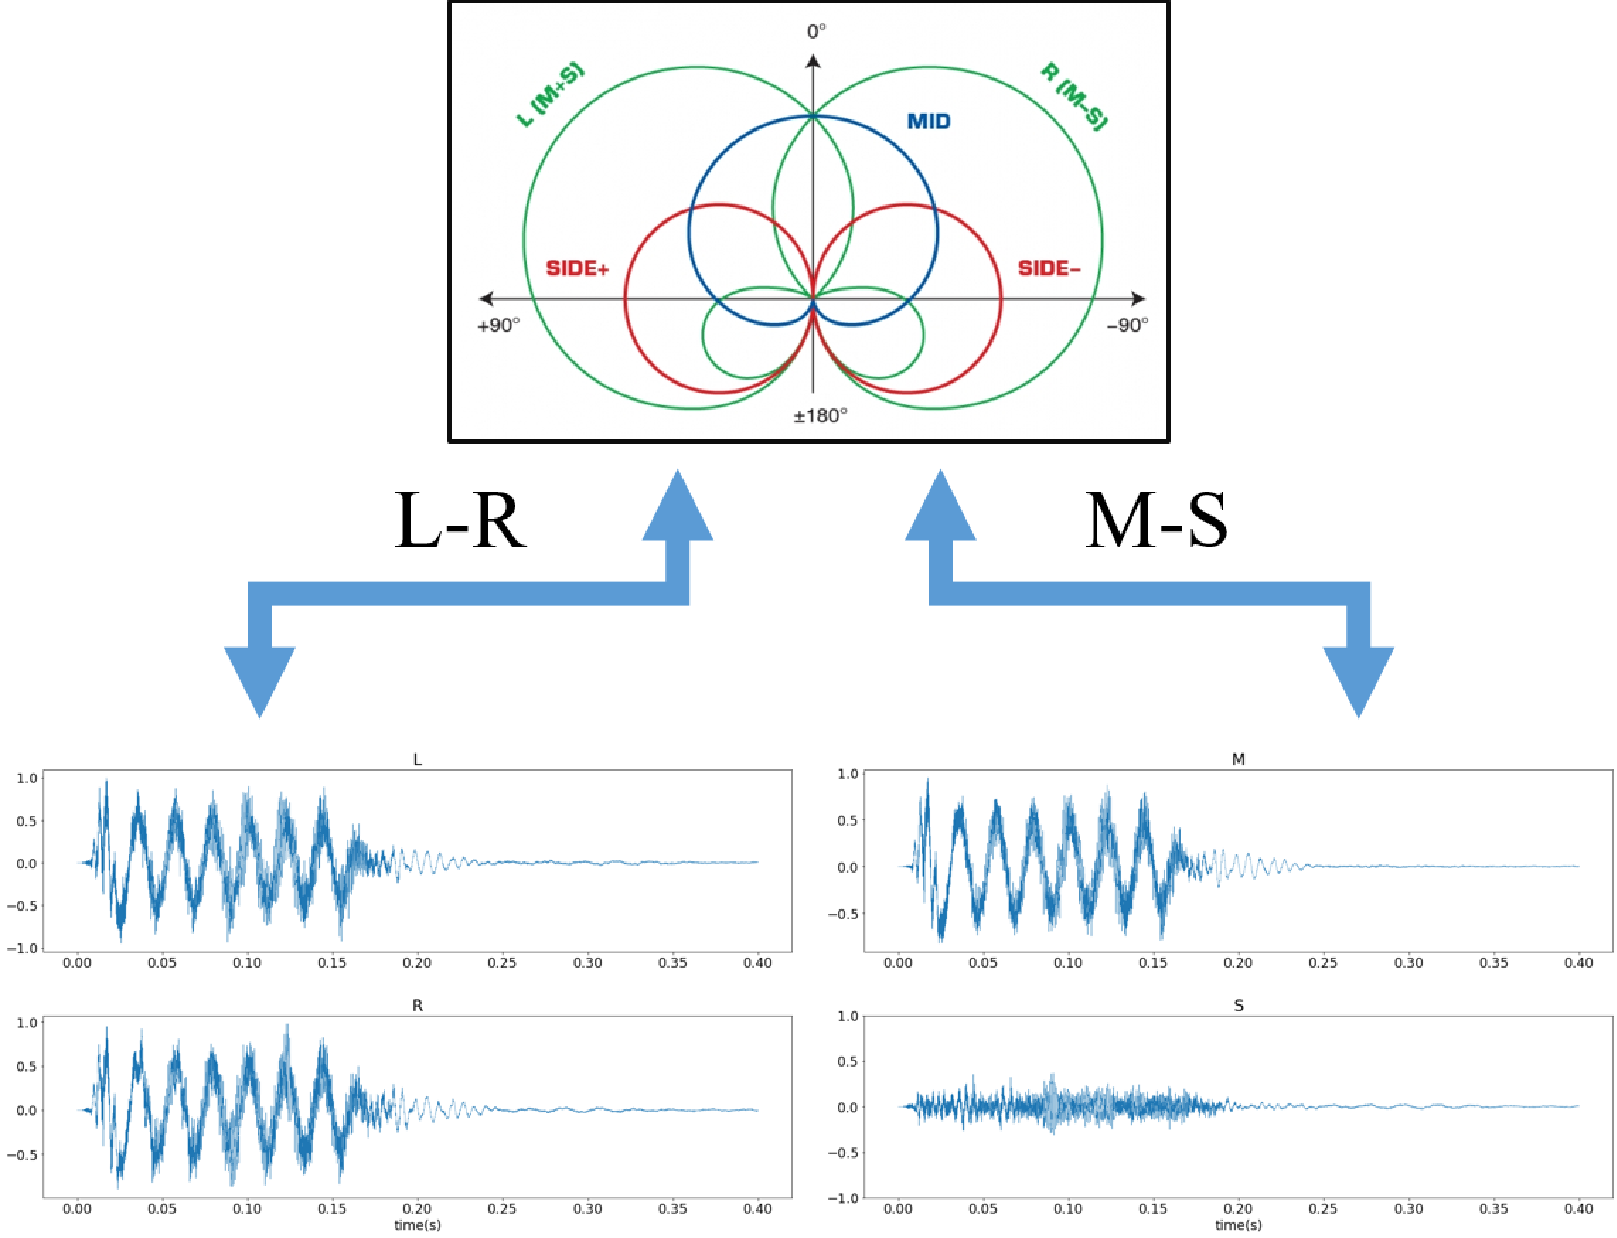
\includegraphics[width=0.85\linewidth]{assets/figures/LRMS.pdf}
    \caption{Example of channel representation for two-channel audio. The left one is the L-R channel representation, and the right one is the M-S channel representation.}
    \label{fig:quality_result}
\end{figure}
As we mentioned above, channel coherency is an important property for the plausible spatiality formation in two-channel audio. However, when the network generates two-channel audio, if left and right channels are created without a guide of channel coherency, the spatiality of the generated audio will not be appropriate. Since creating additional networks associated with channel coherence caused overhead, it is recommended to find a different method to avoid burdening the network. Therefore, it is valid to make the following conjecture: Network will learn stereo image better when using the mid-side (M-S) channel than using the left-right (L-R) channel. When $y$ is stereo audio and $y_M$ and $y_S$ are mid and side channel of stereo audio $y$, $y_M$ and $y_S$ as following:
\begin{equation}
    y_M = {\frac{y_L + y_R}{2}},\quad
    y_S = {\frac{y_L - y_R}{2}}\nonumber
\end{equation}
where $y_L$ and $y_R$ are left and right channel of stereo audio $y$.

\subsection{Custom dataset}
\label{subsec:dataset}
To validate the aforementioned methodology for the stereo image learning for the network, we needed a new dataset. Since we focus on a stereo audio generation model, we needed an audio set with the drastic and various stereo images for our conjecture, but none of the conventional datasets were appropriate. Inspired by the NSynth dataset, which is mainly used by previous studies on neural audio synthesis ~\cite{gansynth, nsynth}, we composed the new dataset using the stab, which is a single staccato note or chord that adds dramatic punctuation to a composition, used in modern electronic music. For clarity of the task, we have adjusted the length of each sample to 400ms. We configured a dataset with a sample rate of 44.1kHz and a bit depth of 16bit.

Since the lack of a large number of our sources, we performed three augmentations to obtain a sufficient amount of data. The augmentation performed are as follows: L-R channel change, time-stretching without pitch shift, and FIR filtering. We produced a total of 11,520 data that maintain the characteristics of the original data through these augmentations. Note that we did not add variations on the pitch because the data often have atonal properties.